\appendix
\clearpage
\section{Appendix}

In Fig.~\ref{fig:power:time:scatter} we plot the E2E time per Epoch in seconds (Y axis) against the Average Power in Watts (X axis). This complements the plot in Fig.~\ref{fig:power:scatter} (same as Fig.~\ref{fig:energy:time:scatter:duplicate}) which reports Total Energy Consumed in milli-Watt hour (mWh). We see an inverse correlation between epoch time and average.

We reproduce Fig.~\ref{fig:power:scatter} from the main text as Fig.~\ref{fig:energy:time:scatter:duplicate} in the appendix. We further plot $4$ variations of this, each highlighting one of the resources changing (core count, CPU frequency, GPU frequency, EMC memory frequency) and the impact each has on the time--energy trade-off and the Pareto front. For each of these plots, we use a group of related markers to highlight a particular resource value, e.g., solid markers for core count 8, hollow markers for core count 4 and line markers for core count 2 in Fig.~\ref{fig:energy:time:cores} where we focus on the effect of CPU cores. Similarly, Fig.~\ref{fig:energy:time:cpuf} shows the effect of CPU frequency, Fig.~\ref{fig:energy:time:gpuf} the effect of GPU frequency and Fig.~\ref{fig:energy:time:memf} the effect of memory frequency.

\claim{Impact of cores}
The number of cores affects the stall time and kernel launch times. However, this is not a significant component of the E2E time for larger models like \mobilenet and \resnet and only affects \lenet noticeably. For instance, the increase in cores from $f$(+) to $e$(\ding{58}) causes a sharp drop in E2E time and energy for \lenet as seen in Fig.~\ref{fig:energy:time:cores}.

\claim{Impact of CPU frequency}
 The CPU frequency affects the stall time and kernel launch time, and therefore has a larger impact on \lenet's E2E time than the other 2 models. This can be seen from Fig.~\ref{fig:energy:time:cpuf}, where the E2E time values for \lenet corresponding to $2265MHz$ (solid red markers with more than $3$ sides) are much lower than those corresponding to $1200MHz$ (hollow red markers), whereas for \resnet and \mobilenet, the E2E time values of the solid green/blue markers are relatively close to those of the hollow green/blue ones.

\claim{Impact of GPU frequency}
Fig.~\ref{fig:energy:time:gpuf} shows the overall impact that GPU frequency has on the different models. GPU frequency affects the GPU compute time, and therefore the E2E time. This impact is more pronounced for compute-intensive models such as \resnet. As seen in Fig.~\ref{fig:energy:time:gpuf}, for \resnet, there is a significant difference in the E2E time values between the data points with a higher GPU frequency of $900MHz$ (indicated by solid green markers with $3$ or $4$ sides) as compared to those with a GPU frequency of $670MHz$ (hollow green markers). This difference is much lesser for \mobilenet, and even more so for \lenet.


\claim{Impact of memory frequency}
Fig.~\ref{fig:energy:time:memf} shows that memory frequency does have an impact on E2E time and energy, but it is not a dominant factor. The impact of memory frequency can only be seen in modes $g$ to $j$, where all other parameters are kept constant. For instance, the increase in memory frequency in going from $h$(+) to $i$($\lozenge$) causes all $3$ models to see a lower E2E time.

\begin{figure}[h!]
\centering

  \centering
	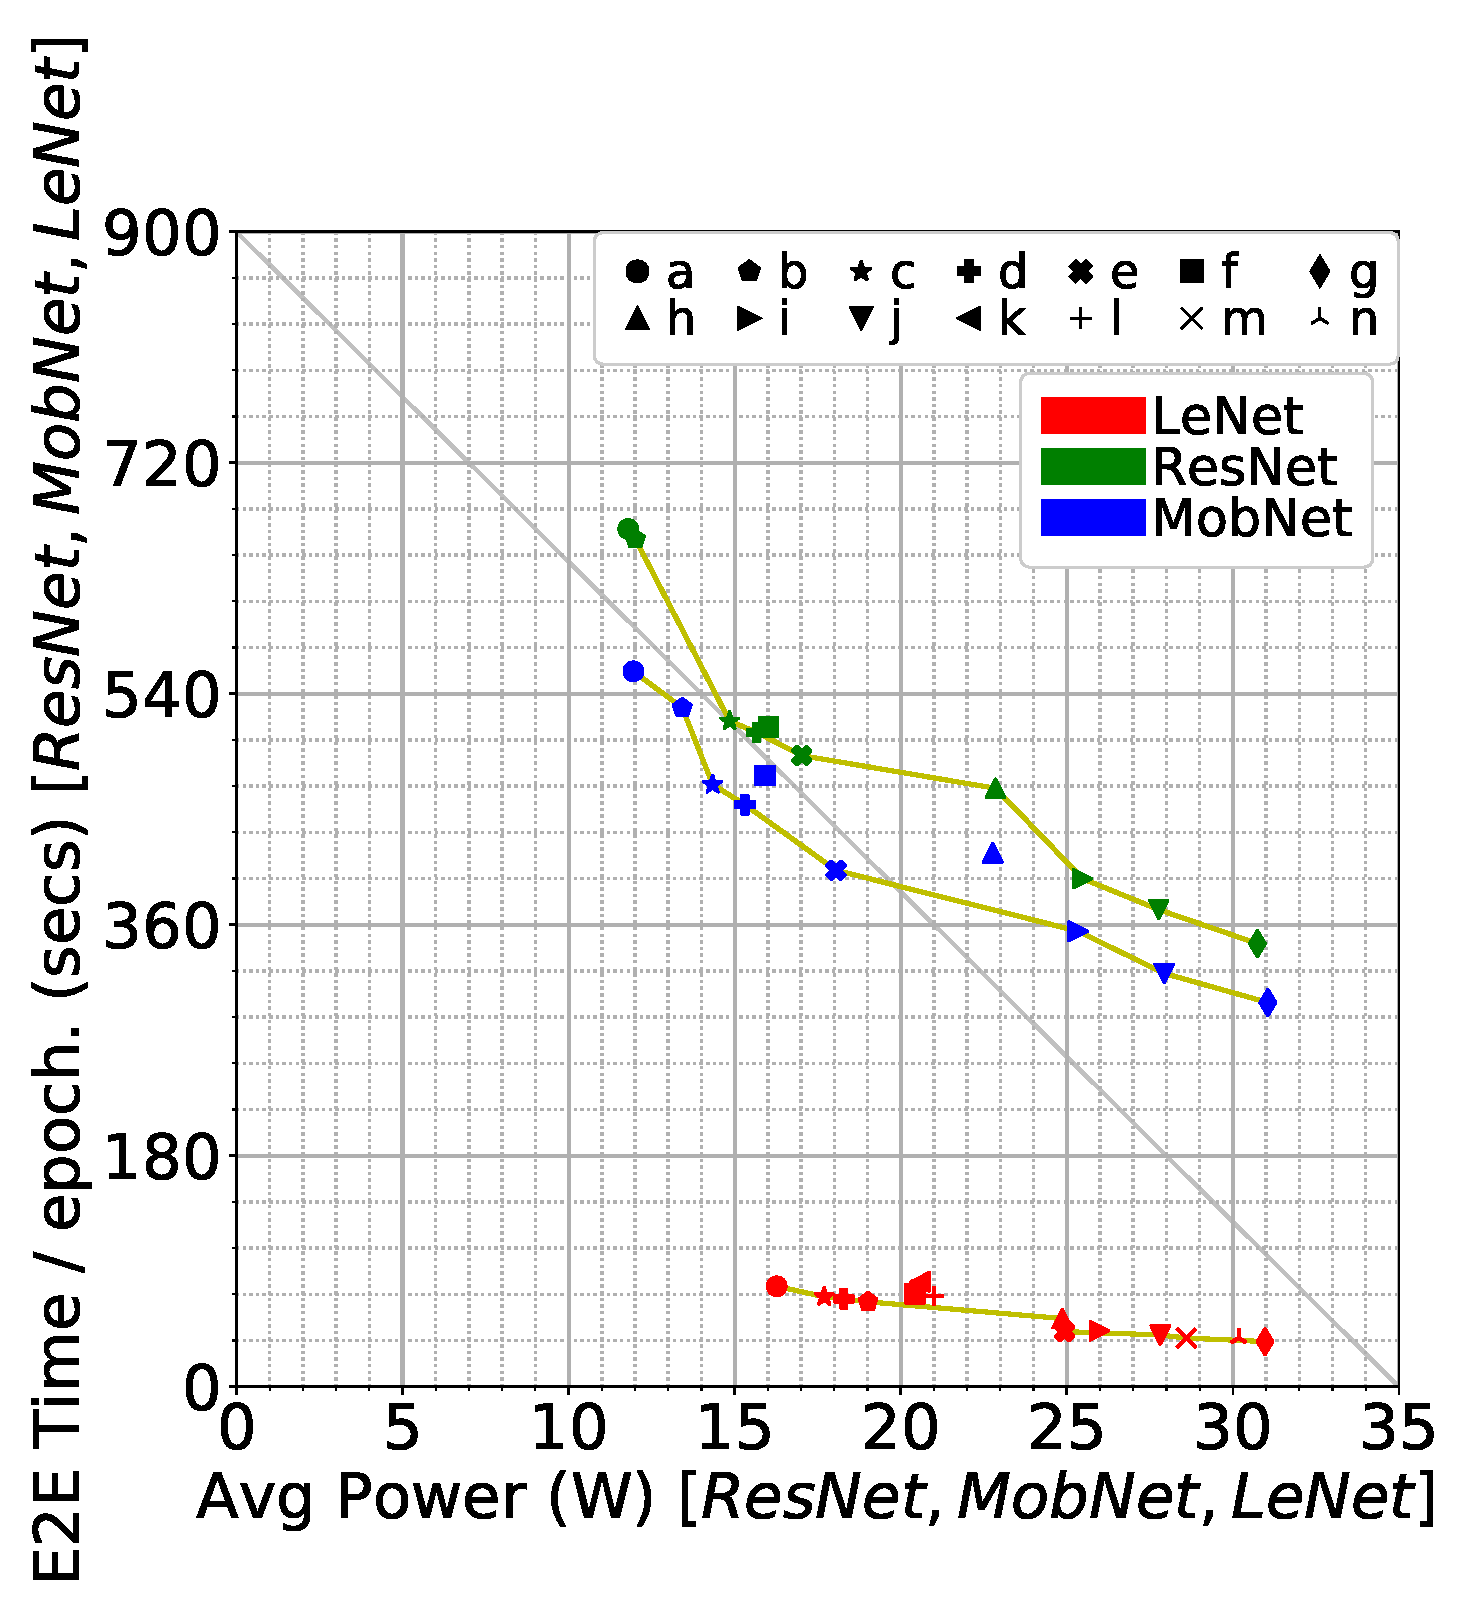
\includegraphics[width=0.5\columnwidth]{images/appendix/power_modes/e2e_power_comparison_all.eps}
\caption{Scatter plot of \textit{E2E time vs. Avg power per epoch ($1+$)}, for power modes $a$--$n$ of AGX for \lenet (secondary axes) and \resnet/\mobilenet (primary axes). The yellow lines indicate the \textit{Pareto front} per DNN.}
\label{fig:power:time:scatter}
\end{figure}

\begin{figure}
  \centering
  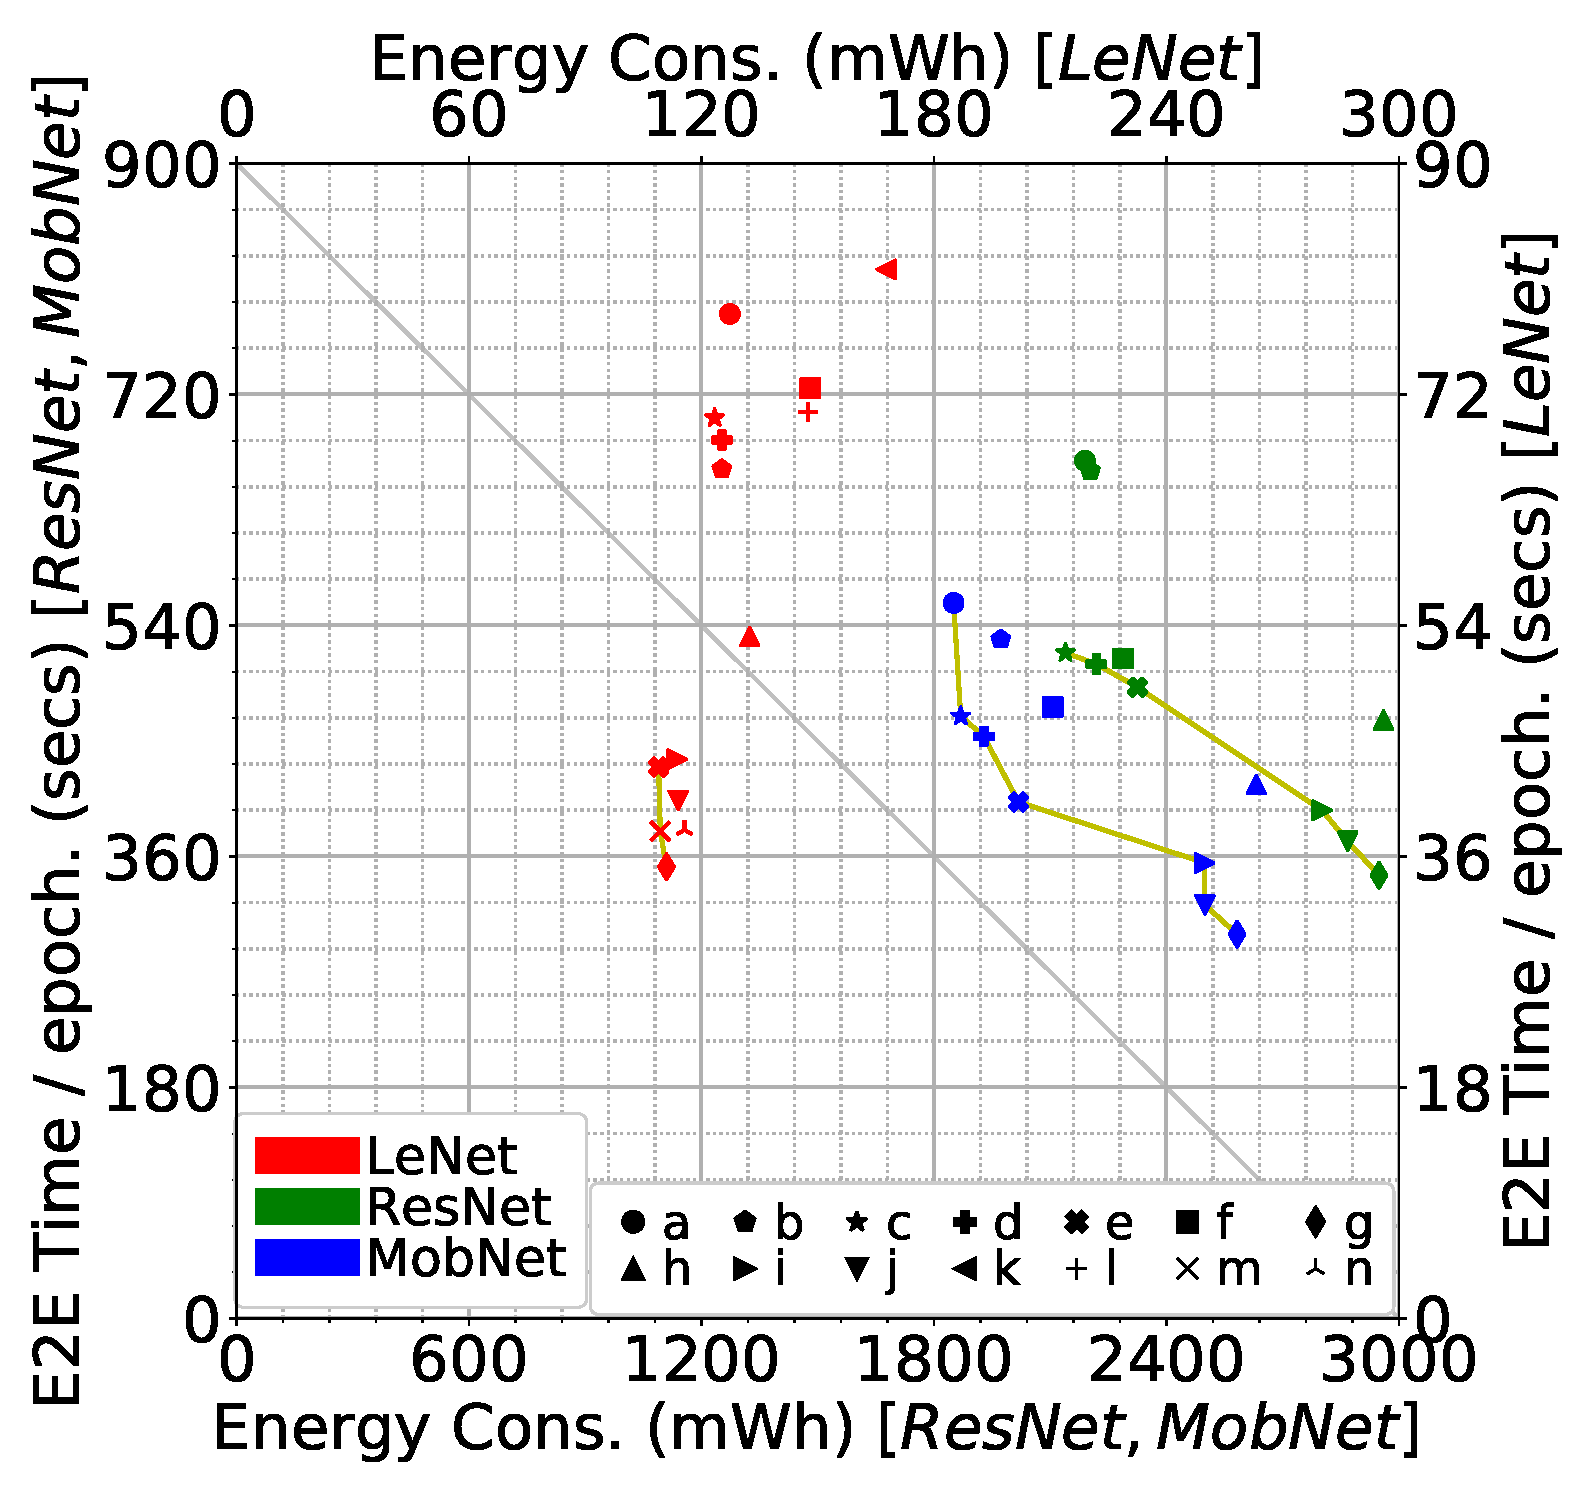
\includegraphics[width=0.5\columnwidth]{images/power_modes/agx/e2e_energy_comparison_all.eps}
% \vspace{-0.2in}
\caption{Scatter plot of \textit{E2E time vs. Energy consumed per epoch ($1+$)}, for power modes $a$--$n$ of AGX for \lenet (secondary axes) and \resnet/\mobilenet (primary axes). The yellow lines indicate the \textit{Pareto front} per DNN. (Same as Fig.~\ref{fig:power:scatter})}
\label{fig:energy:time:scatter:duplicate}
\end{figure}



\begin{figure}
  \centering
	\includegraphics[width=0.5\columnwidth]{images/appendix/power_modes/e2e_energy_cores.eps}
\caption{Scatter plot and Pareto front of \textit{E2E time vs. Energy consumed per epoch ($1+$)} for AGX for \lenet (secondary axes) and \resnet/\mobilenet (primary axes).\\
Markers are grouped by \textbf{CPU Core Count}.
}
\small
\begin{tabular}{c|L{4.2cm}}
\hline
\# Cores & Marker\\
\hline
\hline 
8 & $\bullet$b\quad $\pentagofill$c\quad \ding{72}d\quad \ding{58}e\quad \ding{54}g\quad $\blacksquare$h\quad $\blacklozenge$i\quad $\blacktriangle$j\quad $\RHD$l\quad $\blacktriangledown$m\quad $\LHD$n \\ 
\hline 
4 & $\square$a\quad $\lozenge$k \\
\hline 
2 & +f\\
\hline
\end{tabular}
\label{fig:energy:time:cores}
\end{figure}

%----------------
\begin{figure}
  \centering
	\includegraphics[width=0.5\columnwidth]{images/appendix/power_modes/e2e_energy_cpuf.eps}

\caption{Scatter plot and Pareto front of \textit{E2E time vs. Energy consumed per epoch ($1+$)} for AGX for \lenet (secondary axes) and \resnet/\mobilenet (primary axes).\\
Markers are grouped by \textbf{CPU Frequency}.}

\small
\begin{tabular}{C{3cm}|L{3.8cm}} 
\hline
CPU Freq. (MHz) & Marker \\ 
\hline
\hline
2265 & $\bullet$g\quad $\pentagofill$h\quad \ding{58}i\quad \ding{54}j\quad $\blacksquare$m\quad $\blacklozenge$n\\
\hline
2100 & $\blacktriangle$e\quad $\RHD$f\\
\hline
1200 & $\circ$a\quad $\pentagon$b\quad $\square$c\quad $\lozenge$d\\
\hline
1036 & +k\quad $\times$l\\
\hline
\end{tabular}
\label{fig:energy:time:cpuf}
\end{figure}

\begin{figure}
  \centering
	\includegraphics[width=0.45\columnwidth]{images/appendix/power_modes/e2e_energy_gpuf.eps}
\caption{Scatter plot and Pareto front of \textit{E2E time vs. Energy consumed per epoch ($1+$)} for AGX for \lenet (secondary axes) and \resnet/\mobilenet (primary axes).\\
Markers are grouped by \textbf{GPU Frequency}.}
\small
\begin{tabular}{C{3cm}|L{3.8cm}} 
\hline
GPU Freq. (MHz) & Marker \\ 
\hline
\hline
1377 & $\bullet$g\quad $\pentagofill$h\quad \ding{58}i\quad \ding{54}j\\
\hline
900 & $\blacklozenge$c\quad $\blacktriangle$d\quad $\RHD$e\quad $\blacktriangledown$f\quad $\LHD$n\\
\hline
670 & $\circ$a\quad $\square$b\\
\hline
420 & +k\quad $\times$l\quad $ \curlywedge$m\\
\hline
\end{tabular}
\label{fig:energy:time:gpuf}
\end{figure}

\begin{figure}
  \centering
	\includegraphics[width=0.45\columnwidth]{images/appendix/power_modes/e2e_energy_memf.eps}

\caption{Scatter plot and Pareto front of \textit{E2E time vs. Energy consumed per epoch ($1+$)} for AGX for \lenet (secondary axes) and \resnet/\mobilenet (primary axes).\\
Markers are grouped by \textbf{EMC memory Frequency}.}
\small
\begin{tabular}{C{3cm}|L{3.8cm}} 
\hline
EMC Freq. (MHz) & Marker \\ 
\hline
\hline
2133 & $\bullet$g\quad $\pentagofill$k\quad $\bigstar$l\quad \ding{58}m\quad \ding{54}n\\
\hline
1600 & $\blacksquare$d\quad $\blacklozenge$e\quad $\blacktriangle$f\quad $\RHD$j\\
\hline
1333 & $\circ$a\quad $\pentagon$b\quad $\square$c\quad $\lozenge$i\\
\hline
1066 & +h\\
\hline
\end{tabular}
\label{fig:energy:time:memf}
\end{figure}